% Options for packages loaded elsewhere
\PassOptionsToPackage{unicode}{hyperref}
\PassOptionsToPackage{hyphens}{url}
%
\documentclass[
]{article}
\usepackage{lmodern}
\usepackage{amssymb,amsmath}
\usepackage{ifxetex,ifluatex}
\ifnum 0\ifxetex 1\fi\ifluatex 1\fi=0 % if pdftex
  \usepackage[T1]{fontenc}
  \usepackage[utf8]{inputenc}
  \usepackage{textcomp} % provide euro and other symbols
\else % if luatex or xetex
  \usepackage{unicode-math}
  \defaultfontfeatures{Scale=MatchLowercase}
  \defaultfontfeatures[\rmfamily]{Ligatures=TeX,Scale=1}
\fi
% Use upquote if available, for straight quotes in verbatim environments
\IfFileExists{upquote.sty}{\usepackage{upquote}}{}
\IfFileExists{microtype.sty}{% use microtype if available
  \usepackage[]{microtype}
  \UseMicrotypeSet[protrusion]{basicmath} % disable protrusion for tt fonts
}{}
\makeatletter
\@ifundefined{KOMAClassName}{% if non-KOMA class
  \IfFileExists{parskip.sty}{%
    \usepackage{parskip}
  }{% else
    \setlength{\parindent}{0pt}
    \setlength{\parskip}{6pt plus 2pt minus 1pt}}
}{% if KOMA class
  \KOMAoptions{parskip=half}}
\makeatother
\usepackage{xcolor}
\IfFileExists{xurl.sty}{\usepackage{xurl}}{} % add URL line breaks if available
\IfFileExists{bookmark.sty}{\usepackage{bookmark}}{\usepackage{hyperref}}
\hypersetup{
  hidelinks,
  pdfcreator={LaTeX via pandoc}}
\urlstyle{same} % disable monospaced font for URLs
\usepackage[margin=1in]{geometry}
\usepackage{graphicx,grffile}
\makeatletter
\def\maxwidth{\ifdim\Gin@nat@width>\linewidth\linewidth\else\Gin@nat@width\fi}
\def\maxheight{\ifdim\Gin@nat@height>\textheight\textheight\else\Gin@nat@height\fi}
\makeatother
% Scale images if necessary, so that they will not overflow the page
% margins by default, and it is still possible to overwrite the defaults
% using explicit options in \includegraphics[width, height, ...]{}
\setkeys{Gin}{width=\maxwidth,height=\maxheight,keepaspectratio}
% Set default figure placement to htbp
\makeatletter
\def\fps@figure{htbp}
\makeatother
\setlength{\emergencystretch}{3em} % prevent overfull lines
\providecommand{\tightlist}{%
  \setlength{\itemsep}{0pt}\setlength{\parskip}{0pt}}
\setcounter{secnumdepth}{-\maxdimen} % remove section numbering
\usepackage{setspace}\doublespacing
\usepackage{lineno}\linenumbers

\author{}
\date{\vspace{-2.5em}}

\begin{document}

\hypertarget{estimates-of-phylogenetic-signal-based-on-lambda-are-often-inaccurate}{%
\section{Estimates of Phylogenetic Signal Based on Lambda are Often
Inaccurate}\label{estimates-of-phylogenetic-signal-based-on-lambda-are-often-inaccurate}}

\hfill\break

\textbf{Keywords}: Pagel's lambda, phylogenetic signal \hfill\break

\textbf{Short Title}: Inaccuracies in Pagel's Lambda \hfill\break

\hypertarget{abstract}{%
\section{Abstract}\label{abstract}}

\{conclusion holds: interpreting the regression is not appreciably
different (in terms of slopes and f values)\}

\newpage

\hypertarget{introduction}{%
\section{Introduction}\label{introduction}}

Investigating macroevolutionary patterns of trait variation requires a
phylogenetic perspective, because the shared ancestry among species
generates statistical non-independence (Felsenstein 1985; Harvey and
Pagel 1991). Accounting for this evolutionary non-independence is the
purview of \emph{phylogenetic comparative methods} (PCMs); a suite of
analytical tools that condition the data on the phylogeny through the
course of statisical evaluations of phenotypic trends (e.g., Grafen
1989; Garland and Ives 2000; Rohlf 2001; Butler and King 2004). The past
several decades have witnessed a rapid expansion in the development of
PCMs to address an ever-growing set of macroevolutionary hypotheses
(Martins and Hansen 1997; O'Meara et al. 2006; Revell and Harmon 2008;
Beaulieu et al. 2012; Adams 2014b,a; Adams and Collyer 2018). These
methods are predicated on the notion that phylogenetic signal -- the
tendancy for closely related species to display similar trait values --
is present in cross-species datasets (Felsenstein 1985; Pagel 1999;
Blomberg et al. 2003). Indeed, under numerous evolutionary models,
phylogenetic signal is to be expected, as stochastic character change
along the hierarchical structure of the tree of life generates trait
covaration among related taxa (see Felsenstein 1985; Blomberg et al.
2003; Revell et al. 2008). \hfill\break

For many macroevolutionary analyses, it is often of interest to quantify
the degree to which phylogenetic signal is displayed in continuous
traits. Several analytical tools have been developed for this purpose
(e.g., Gittleman and Kot 1990; Abouheif 1999; Pagel 1999; Blomberg et
al. 2003; Klingenberg and Gidaszewski 2010; Adams 2014a), which differ
primarily in how they characterize the phylogenetic dependency of trait
variation among taxa. One commonly used statistical measure,
\emph{Kappa} (\(K\)), expresses the strength of phylogenetic signal as
the ratio of observed trait variation to the trait variation conditioned
on the phylogeny; which is then scaled by what is expected under
Brownian motion given the phylogeny's size and shape (Blomberg et al.
2003; also Adams 2014a). Another approach, Pagel's \(\lambda\) (Pagel
1999), uses maximum likelihood to fit the data to the phylogeny under
some model of evolutionary change (typically Brownian motion). The
inclusion of a scaling parameter, \(\lambda\), transforms the lengths of
the internal branches of the phylogeny to improve the fit, and this
parameter describes the degree of phylogenetic signal in the dataset
(Pagel 1999; Freckleton et al. 2002). Pagel's \(\lambda\) also has the
appeal that it may be included when estimating the association of traits
in a phylogenetic context, meaning that one may account for the degree
of phylogenetic signal while conducting phylogenetic regression or ANOVA
(see Freckleton et al. 2002). \hfill\break

Several studies have investigated the statistical properties of methods
for estimating phylogenetic signal under various conditions (e.g.,
Munkemuller et al. 2012; Pavoine and Ricotta 2012; Diniz-Filho et al.
2012; Molina-Venegas and Rodriguez 2017; see also Revell et al. 2008;
Revell 2010). These have largely focused on the ability of methods to
detect the presence of phylogenetic signal (i.e., type I and type II
error rates) under complex models of evolutionary change, across a range
of phylogeny sizes, and with varying degrees of phylogenetic uncertainty
or unresolved topologies. In terms of parameter estimation, Revell
(2010) found that regression parameters were accurately estimated when
\(\lambda\) was included during phylogenetic regression, and Munkmuller
et al.~(2012) demonstrated that estimates of phylogenetic signal
obtained using various measures generally increased when input levels of
phylogenetic signal were stronger. However, the precision of those
estimates could not be determined, because the input levels of
phylogenetic signal were simulated via a scaling factor (\(w\)) that was
not directly comparable to the measures of phylogenetic signal being
compared (see Munkemuller et al. 2012). Indeed, understanding the
precision in estimating levels of phylogenetic signal is paramount,
because biological inferences regarding the strength of phylogenetic
signal in phenotypic datasets requires high precision of its estimation.
One study (Boettiger et al. 2012) found that estimates of Pagel's
\(\lambda\) displayed less variation when data were simulated on a large
phylogeny (\(N=281\)) as compared to a small one (\(N=13\)), concluding
that insufficient data (i.e., the number of species) was the underlying
cause of the increased variation across parameter estimates. However,
this conclusion assumes that the precision in estimating \(\lambda\)
remains constant across its range (\(\lambda = 0 \to 1\)); an assumption
that to date, has not been verified. Thus, despite widespread use of
Pagel's (1999) \(\lambda\) in macroevolutionary studies, at present, we
still lack a general understanding of the precision with which
\(\lambda\) can estimate levels of phylogenetic signal in phenotypic
datasets. \hfill\break

In this study, we evaluate the precision of Pagel's \(\lambda\) in
estimating known levels of phylogenetic signal in phenotypic data. We
use computer simulations with differing numbers of species, differently
shaped phylogenies, and differing input levels of phylogenetic signal,
to explore the degree to which \(\lambda\) correctly identifies known
levels of phylogenetic signal, and under what circumstances. We also
evaluate the precision of a standardized effect size (\(Z_K\)) based on
\(Kappa\) for comparison. Additionally, we use simulations to determine
how the inclusion of \(\lambda\) in phylogenetic regression and ANOVA
(i.e., PGLS) affects parameter estimation, and whether levels of
phylogenetic signal estimated in a PGLS framework are accurate. We then
survey the recent macroevolutionary literature for published papers
containing estimates of \(\lambda\) from empirical datasets, and compare
these empirical estimates to patterns gleaned from our computer
simulations. In general we find that while PGLS parameters (e.g.,
\(\beta\)) are accurately estimated with the inclusion of phylogenetic
signal, estimates of \(\lambda\) are not. We also find that estimates of
\(\lambda\) vary widely for a given input value of phylogenetic signal,
and that this variation is not constant across the range of input
signal, with decreased precision when phylogenetic signal is of
intermediate strength. Additionally, the same \(\lambda_{est}\) may be
obtained from datasets containing vastly different input levels of
phylogenetic signal. By contrast, variation across effect sizes
(\(Z_K\)) obtained from \(Kappa\) is far more consistent across the
range of input values, and the precision of \(Z_K\) is generally
preferable to that of \(\lambda_{est}\). Further, because \(Z_K\) is a
standardized effect size, the strength of phylogenetic signal is more
readily interpretable, and may be compared across datasets. We conclude
that estimates of phylogenetic signal using Pagel's \(\lambda\) are
often inaccurate, and thus interpreting strength of phylogenetic signal
in phenotypic datasets based on this measure is compromised. By
contrast, effect sizes obtained from \(Kappa\) hold promise for
characterizing phylogenetic signal, and for comparing the strength of
phylogenetic signal across datasets.

\hypertarget{materials-and-methods}{%
\section{Materials and Methods}\label{materials-and-methods}}

\hypertarget{simulations}{%
\subsection{\texorpdfstring{\emph{Simulations}}{Simulations}}\label{simulations}}

We conducted a series of computer simulations to evaluate the ability of
Pagel's \(\lambda\) to estimate known levels of phylogenetic signal. Our
primary simulations were based on pure-birth phylogenies; however, we
also evaluated patterns on both balanced and pectinate trees to
determine whether tree shape affected our findings (see Supporting
Information). Our first set of simulations evaluated the extent to which
values of \(\lambda\) estimated from the data corresponded with actual
input levels of phylogenetic signal. For these simulations we generated
50 pure-birth phylogenies at each of six different tree sizes, ranging
from 32 to 1024 taxa (\(n=2^5 - 2^{10}\)). Next, we rescaled the
simulated phylogenies by multiplying the internal branches by
\(\lambda\). We used a set of values that encompassed the entire range
of \(\lambda\): (\(\lambda_{in} = 0.0 \to 1.0\); in 21 intervals of 0.05
units), resulting in 1050 scaled phylogenies at each level of species
richness (\(n\)). Continuous traits were then simulated on each
phylogeny under a Brownian motion model of evolution to obtain datasets
with known and differing levels of phylogenetic signal. These varied
from datasets with no phylogenetic signal (when \(\lambda_{in} =0\)) to
datsets with phylogenetic signal corresponding to what was expected
under Brownian motion (when \(\lambda_{in} =1\)). \hfill\break

Using the simulated phylogenies we estimated the phylogenetic signal in
each dataset using Pagel's \(\lambda\). Next, for the 1050 datasets at
each level of species richness (\(n\)), we assessed the relationship
between \(\lambda_{in}\) and \(\lambda_{est}\) using regression.
Additionally, the precision of \(\lambda\) was approximated by observing
the variation of \(\lambda_{est}\) obtained at each input level of
phylogenetic signal (\(\lambda_{in}\)). Finally, for comparison we
characterized the strength of phylogenetic signal in each dataset using
a standardized effect size (\(Z_K\): sensu Adams and Collyer 2016,
2019a) based on \(Kappa\). As suggested by Adams and Collyer (2019b), an
effect size for phylogenetic signal may be estimated as:
\(Z_K=\frac{K_{obs}-\mu_K}{\sigma_K}\), where \(K_{obs}\) was the
observed \(Kappa\), and \(\mu_K\) and \(\sigma_K\) were the mean and
standard deviation of the empirical sampling distribution of values
obtained from the permutation distribution. \(Z_K\) describes the
strength of phylogenetic signal as a standard deviate from its sampling
distribution, and thus directly measures the strength of signal in a
manner that is comparable across datasets. Variation in the set of
\(Z_K\) at each input level of phylogenetic signal was then calculated
as an estimate of precision in \(Z_K\). However, because \(Z_K\) differs
in scale from \(\lambda\), we used a linear normalization to standardize
\(Z_K\) to a uniform distribution (\(0\rightarrow1\)), and estimated the
precision of \(Z_K\) from the normalized values. \hfill\break

Our second set of simulations evaluated the extent to which values of
\(\lambda\) estimated in PGLS regression and ANOVA (i.e., \(Y\sim{X}\))
corresponded with actual input levels of phylogenetic signal in the
response variable. As before we generated 50 pure-birth phylogenies at
each of six levels of species richness (\(n=2^5 - 2^{10}\)), and
rescaled each with a set of input \(\lambda\) values
(\(\lambda_{in} = 0.0 - 1.0\); in 21 intervals of 0.05 units). Next, an
independent variable \(X\) was simulated on each phylogeny under a
Brownian motion model of evolution (for PGLS regression). For
phylogenetic ANOVA, random groups (\(X\)) were obtained by simulating a
discrete (binary) character on each phylogeny. Next, the dependent
variable was simulated in such a manner as to contain a known
relationship with \(X\) plus random error containing phylogenetic
signal. This was accomplished as: \(Y=\beta{X}+\epsilon\). Here, the
association between \(Y\) and \(X\) was modeled using a range of values:
\(\beta=(0.0,0.25, 0.5, 0.75,1.0)\), and the residual error was modeled
to contain phylogenetic signal simulated under a Brownian motion model
of evolution: \(\epsilon=\mathcal{N}(\mu=0,\sigma=\mathbf{C})\): (see
Revell 2010 for a similar simulation design). For each dataset, the fit
of the phylogenetic regression was estimated using maximum likelihood,
and parameter estimates (\(\beta_{est}\) and \(\lambda_{est}\)) were
obtained and evaluated as above. All analyses were performed in R v3.6.0
(R Core Team 2019) using the packages \texttt{geiger} (Harmon et al.
2008), \texttt{caper} (Orme et al. 2013), \texttt{phytools} (Revell
2012), and \texttt{geomorph} (Adams and Otárola-Castillo 2013; Adams et
al. 2020). R-scripts are found in the Supporting Information.

\hypertarget{literature-survey}{%
\subsection{\texorpdfstring{\emph{Literature
Survey}}{Literature Survey}}\label{literature-survey}}

To determine how Pagel's \(\lambda\) is commonly utilized in empirical
studies, we conducted a literature survey. From Google.scholar we
obtained a list of all papers published in 2019 that used \(\lambda\);
resulting in 341 studies. For each study, we extracted all
\(\lambda_{est}\), the size of the phylogeny (\(n\)), and noted whether
authors reported confidence intervals or performed significance tests
assessing difference of \(\lambda_{est}\) from either zero or one. We
also noted whether biological interpretations based on \(\lambda_{est}\)
were made, and for studies that reported more than one
\(\lambda_{est}\), we also noted whether these were compared in some
manner, and whether such comparisons were accompanied with statistical
tests between \(\lambda_{est}\).

\hypertarget{results}{%
\section{Results}\label{results}}

\hypertarget{simulations-1}{%
\subsection{\texorpdfstring{\emph{Simulations}}{Simulations}}\label{simulations-1}}

Our first set of simulations revealed several patterns. First, the
relationship between \(\lambda_{est}\) and \(\lambda_{in}\) across the
range input levels of phylogenetic signal was \(\beta\sim1.0\);
indicating that the average \(\lambda_{est}\) across datasets for a
given simulation condition correctly reflected the input levels of
phylogenetic signal. However, as shown in Figure 1, the precision of
those estimates varied widely, and in several interesting ways.
Predictably, precision was worse at low levels of species richness,
where in many cases the set of \(\lambda_{est}\) spanned nearly the
entire range of possible values (e.g., \(n=32\); \(\lambda_{in}=0.5\):
range of \(\lambda_{est}= 0.0\to 0.985\)). Second, as species richness
increased, variation across estimates of \(\lambda\) decreased (Figure
1). This confirmed the pattern identified by Boettiger et al.~(2012) on
a small (\(n=13\)) versus a large (\(n=281\)) phylogeny, and
demonstrated that the trend of increasing precision with higher species
richness was general; adhering to parametric statistical theory.
Importantly however, our broader set of simulations revealed that the
precision of \(\lambda_{est}\) was not uniform across all levels of
phylogenetic signal. Specifically, we found that variation in
\(\lambda_{est}\) was highest at intermediate levels of phylogenetic
signal, and decreased at both lower and higher levels of input signal
(Figure 1). This implied that the precision in estimating \(\lambda\)
was worse at intermediate values, and improved as the levels of
phylogenetic signal were closer to \(\lambda_{in}=0\) (no phylogenetic
signal) or \(\lambda_{in}=1\) (Brownian motion). Notably, even at large
levels of species richness, the range of \(\lambda_{est}\) still
encompassed a substantial portion of possible values (e.g., \(n=512\);
\(\lambda_{in}=0.5\): range of \(\lambda_{est} = 0.32\to 0.68\)).
Likewise, the same \(\lambda_{est}\) could be obtained from datasets
containing vastly different input levels of phylogenetic signal (e.g.,
\(n=512\); \(\lambda_{est} = 0.5\); range of
\(\lambda_{in} = 0.25 \to 0.65\)). Taken together, these findings reveal
that \(\lambda_{est}\) does not precisely characterize observed levels
of phylogenetic signal in phenotypic datasets, and that biological
interpretations of the strength of phylogenetic signal based on
\(\lambda\) may be highly inaccurate. \hfill\break

{[}insert Figure 1 here{]} \hfill\break

By contrast, when characterizing phylogenetic signal with the
standardized effect size (\(Z_K\)) of \(Kappa\), we found that the
precision of \(Z_K\) was more stable, as variation across datasets was
far more consistent across the range of input values. For example, when
\(n=128\) the precision of \(\lambda_{est}\) (Figure 2A) varied
considerably more across input levels of phylogenetic signal than did
the precision of \(Z_K\) for the same datasets (Figure 2B). Further, for
a given \(n\), the variance in precision estimates of \(Z_K\) was
considerably smaller than the variance in precision estimates of
\(\lambda_{est}\) (Fig. 2C,D); implying that estimates of phylogenetic
signal were more reliable and robust when using \(Z_K\) (for additional
results see Supporting Information). Finally, it should also be
recognized that because \(Z_K\) is a standardized effect size, the
strength of phylogenetic signal is more readily interpretable when using
this measure, as \(Z_K\) expresses the strength of phylogenetic signal
in standard deviation units relative to the mean (see Adams and Collyer
2019b). This further implies that comparisons of the strength of
phylogenetic signal among phenotypic traits are possible, and may be
accomplished statistically via a two-sample test that formally compares
\(Z_K\) across datasets (for comparisons of multivariate effect sizes
see: Adams and Collyer 2016, 2019a). \hfill\break

{[}insert Figure 2 here{]} \hfill\break 

When \(\lambda\) was incorporated in PGLS regression and ANOVA (i.e.,
\(Y\sim{X}\)), we found much the same pattern as in our earlier
simulations. Namely, the precision of \(\lambda_{est}\) covaried with
species richness; where greater precision was obtained at higher levels
of species richness (Figure 3). Likewise, the precision in estimating
\(\lambda\) was worse at intermediate values (Figure 3), and improved as
the levels of phylogenetic signal were closer to \(\lambda_{in}=0\) (no
phylogenetic signal) or \(\lambda_{in}=1\) (Brownian motion). Generally,
the spread of estimates was slightly broader when \(\lambda\) was
co-estimated with regression parameters in PGLS regression (Figure 3),
as compared to when \(\lambda\) was estimated for only the dependent
variable (Figure 1). Finally, we found that regression parameters
(\(\beta\)) were accurately estimated when \(\lambda\) was included
during phylogenetic regression; a result which confirmed earlier
findings of Revell (2010) (see Supporting Information). \hfill\break

{[}insert Figure 3 here{]}

\hypertarget{literature-survey-1}{%
\subsection{\texorpdfstring{\emph{Literature
Survey}}{Literature Survey}}\label{literature-survey-1}}

We found 182 manuscripts from 2019 that estimated and reported Pagel's
lambda values using PGLS methods. These papers averaged 8.527 lambda
values, ranging from a single lambda estimate up to 71 estimated
lambdas. Almost exactly half of the published lambda estimates were
either below 0.05 (25.32\%) or above 0.9 (24.74\%; Figure 3). 73.32\% of
the published lambdas were estimated using phylogenies with fewer than
200 tips, and 348 lambda estimates (8.57\% of all published estimates)
came from phylogenies with fewer than 30 tips. \hfill\break

{[}insert Figure 4 here{]} \hfill\break

Many of the reviewed manuscripts liberally interpreted the magnitude of
the estimate lambda, using phrases such as ``strong'' or ``weak''
phylogentic signal when statistically, all that was clear was a
difference between the estimated lambda and 0 or 1 respectively. We
estimated that about 20.49\% of the manuscripts revealed some sort of
biological interpretation of the magnitude of estimated phylogenetic
signal that overreached the statistical findings. We also identified
seven manuscripts as having inappropriately interpreted differences in
lambda values, indicating that some traits had stronger or weaker signal
than other traits without the appropriate statistical tests.
\hfill\break

As is evidenced by macroevolutionary papers published in 2019 papers,
Pagel's lambda estimation methods are often misused and
over-interpretted. Despite the urging of Boettiger and colleagues to
publish confidence intervals with all lambda parameter estimates, only
18\% of papers published in 2019 do so.

\hypertarget{results-1}{%
\section{Results}\label{results-1}}

\hypertarget{discussion}{%
\section{Discussion}\label{discussion}}

1: summary paragraph

2: expand on Lambda.. lambda innacurate, not precise, level of precision
varies with input physig (worse in mid-range). NEW RESULT. We are first
to show this. NOTE: pattern is obvious with reflection. Since it is a
`bounded' parameter estimation should be best at the extremes\ldots{}
(state this?).. hmm.

Patterns worse with PGLS, though beta still estimated properly.
Conclusion, lambda not overly useful.

3: By contrast, effect size Z-K useful, equally precise across range of
values. Can be used to characterize the strength of physignal, and
because robust to input levels, etc. may be used to compare across
datasets.

Somewhere, recognize that this is somewhat `backwards' from prior
recommendations where Kappa had somewhat lower performance in terms of
type I and type II error (which?? I forget). However, recall that those
studies did not examine the precision of the estimates. Nor was Z-k
included, because it was not yet invented. So Use of Z-k should make
good sense here.

Closing paragraph.

\hfill\break

More discussion paragraphs

\newpage

\hypertarget{references}{%
\section{References}\label{references}}

\setlength{\parindent}{-0.25in} \setlength{\leftskip}{0.25in}
\setlength{\parskip}{8pt} \noindent

\hypertarget{refs}{}
\leavevmode\hypertarget{ref-Abouheif1999}{}%
Abouheif, E. 1999. A method for testing the assumption of phylogenetic
independence in comparative data. Evolutionary Ecology Research
1:895--909.

\leavevmode\hypertarget{ref-Adams2014a}{}%
Adams, D. C. 2014a. A generalized Kappa statistic for estimating
phylogenetic signal from shape and other high-dimensional dultivariate
data. Systematic Biology 63:685--697.

\leavevmode\hypertarget{ref-Adams2014b}{}%
Adams, D. C. 2014b. A method for assessing phylogenetic least squares
models for shape and other high-dimensional multivariate data. Evolution
68:2675--2688.

\leavevmode\hypertarget{ref-AdamsCollyer2019b}{}%
Adams, D. C., and M. L. Collyer. 2019a. Comparing the strength of
modular signal, and evaluating alternative modular hypotheses, using
covariance ratio effect sizes with morphometric data. Evolution
73:2352--2367.

\leavevmode\hypertarget{ref-AdamsCollyer2016}{}%
Adams, D. C., and M. L. Collyer. 2016. On the comparison of the strength
of morphological integration across morphometric datasets. Evolution
70:2623--2631.

\leavevmode\hypertarget{ref-AdamsCollyer2018b}{}%
Adams, D. C., and M. L. Collyer. 2018. Phylogenetic anova: Group-clade
aggregation, biological challenges, and a refined permutation procedure.
Evolution 72:1204--1215.

\leavevmode\hypertarget{ref-AdamsCollyer2019}{}%
Adams, D. C., and M. L. Collyer. 2019b. Phylogenetic comparative methods
and the evolution of multivariate phenotypes. Annual Review of Ecology,
Evolution, and Systematics 50:405--425.

\leavevmode\hypertarget{ref-AdamsGeomorph}{}%
Adams, D. C., M. L. Collyer, and A. Kaliontzopoulou. 2020. Geomorph:
Software for geometric morphometric analyses. R package version 3.2.1.

\leavevmode\hypertarget{ref-AdamsOtarola2013}{}%
Adams, D. C., and E. Otárola-Castillo. 2013. Geomorph: An r package for
the collection and analysis of geometric morphometric shape data.
Methods in Ecology and Evolution 4:393--399.

\leavevmode\hypertarget{ref-Beaulieu_et_al2012}{}%
Beaulieu, J. M., D. C. Jhwueng, C. Boettiger, and B. C. O'Meara. 2012.
Modeling stabilizing selection: Expanding the ornstein-uhlenbeck model
of adaptive evolution. Evolution 66:2369--2383.

\leavevmode\hypertarget{ref-Blomberg_et_al2003}{}%
Blomberg, S. P., T. Garland, and A. R. Ives. 2003. Testing for
phylogenetic signal in comparative data: Behavioral traits are more
labile. Evolution 57:717--745.

\leavevmode\hypertarget{ref-Boettiger_et_al2012}{}%
Boettiger, C., G. Coop, and P. Ralph. 2012. Is your phylogeny
informative? Measuring the power of comparative methods. Evolution
67:2240--2251.

\leavevmode\hypertarget{ref-ButlerKing2004}{}%
Butler, M. A., and A. A. King. 2004. Phylogenetic comparative analysis:
A modeling approach for adaptive evolution. American Naturalist
164:683--695.

\leavevmode\hypertarget{ref-DinizFilho2012}{}%
Diniz-Filho, J. A. F., T. Santos, T. F. Rangel, and L. M. Bini. 2012. A
comparison of metrics for estimating phylogenetic signal under
alternative evolutionary models. Genetics and Molecular Biology
35:673--679.

\leavevmode\hypertarget{ref-Felsenstein1985}{}%
Felsenstein, J. 1985. Phylogenies and the comparative method. American
Naturalist 125:1--15.

\leavevmode\hypertarget{ref-Freckleton_et_al2002}{}%
Freckleton, R. P., P. H. Harvey, and M. Pagel. 2002. Phylogenetic
analysis and comparative data: A test and review of evidence. American
Naturalist 160:712--726.

\leavevmode\hypertarget{ref-GarlandIves2000}{}%
Garland, T. J., and A. R. Ives. 2000. Using the past to predict the
present: Confidence intervals for regression equations in phylogenetic
comparative methods. American Naturalist 155:346--364.

\leavevmode\hypertarget{ref-Gittleman1990}{}%
Gittleman, J. L., and M. Kot. 1990. Adaptation: Statistics and a null
model for estimating phylogenetic effects. Systematic Zoology
39:227--241.

\leavevmode\hypertarget{ref-Grafen1989}{}%
Grafen, A. 1989. The phylogenetic regression. Philosophical Transactions
of the Royal Society of London B, Biological Sciences 326:119--157.

\leavevmode\hypertarget{ref-Harmon2008}{}%
Harmon, L. J., J. T. Weir, C. D. Brock, R. E. Glor, and W. Challenger.
2008. GEIGER: Investigating evolutionary radiations. Bioinformatics
24:129--131.

\leavevmode\hypertarget{ref-HarveyPagel1991}{}%
Harvey, P. H., and M. D. Pagel. 1991. The comparative method in
evolutionary biology. Oxford University Press, Oxford.

\leavevmode\hypertarget{ref-Klingenberg2010}{}%
Klingenberg, C. P., and N. A. Gidaszewski. 2010. Testing and quantifying
phylogenetic signals and homoplasy in morphometric data. Systematic
biology 59:245--261.

\leavevmode\hypertarget{ref-MartinsHansen1997}{}%
Martins, E. P., and T. F. Hansen. 1997. Phylogenies and the comparative
method: A general approach to incorporating phylogenetic information
into the analysis of interspecific data. American Naturalist
149:646--667.

\leavevmode\hypertarget{ref-MolinaVenegas2017}{}%
Molina-Venegas, R., and M. A. Rodriguez. 2017. Revisiting phylogenetic
signal; strong or negligible impacts of polytomies and branch length
information? BMC evolutionary biology 17:53.

\leavevmode\hypertarget{ref-Munkemuller_et_al2012}{}%
Munkemuller, T., S. Lavergne, B. Bzeznik, S. Dray, T. Jombart, K.
Schiffers, and W. Thuiller. 2012. How to measure and test phylogenetic
signal. Methods in Ecology and Evolution 3:743--756.

\leavevmode\hypertarget{ref-OMeara_et_al2006}{}%
O'Meara, B. C., C. Ane, M. J. Sanderson, and P. C. Wainwright. 2006.
Testing for different rates of continuous trait evolution using
likelihood. Evolution 60:922--933.

\leavevmode\hypertarget{ref-Orme2013}{}%
Orme, D., R. P. Freckleton, G. H. Thomas, T. Petzoldt, S. A. Fritz, and
N. Isaac. 2013. CAPER: Comparative analyses of phylogenetics and
evolution in r. Methods in Ecology and Evolution 3:145--151.

\leavevmode\hypertarget{ref-Pagel1999}{}%
Pagel, M. D. 1999. Inferring the historical patterns of biological
evolution. Nature 401:877--884.

\leavevmode\hypertarget{ref-Pavoine2012}{}%
Pavoine, S., and C. Ricotta. 2012. Testing for phylogenetic signal in
biological traits: The ubiquity of cross-product statistics. Evolution:
International Journal of Organic Evolution 67:828--840.

\leavevmode\hypertarget{ref-RCT}{}%
R Core Team. 2019. R: A language and environment for statistical
computing. R Foundation for Statistical Computing, Vienna, Austria.

\leavevmode\hypertarget{ref-Revell2010}{}%
Revell, L. J. 2010. Phylogenetic signal and linear regression on species
data. Methods in Ecology and Evolution 1:319--329.

\leavevmode\hypertarget{ref-Revell2012}{}%
Revell, L. J. 2012. Phytools: An r package for phylogenetic comparative
biology (and other things). Methods in Ecology and Evolution 3:217--223.

\leavevmode\hypertarget{ref-RevellHarmon2008}{}%
Revell, L. J., and L. J. Harmon. 2008. Testing quantitative genetic
hypotheses about the evolutionary rate matrix for continuous characters.
Evolutionary Ecology Research 10:311--331.

\leavevmode\hypertarget{ref-Revell_et_al2008}{}%
Revell, L. J., L. J. Harmon, and D. C. Collar. 2008. Phylogenetic
signal, evolutionary process, and rate. Systematic Biology 57:591--601.

\leavevmode\hypertarget{ref-Rohlf2001}{}%
Rohlf, F. J. 2001. Comparative methods for the analysis of continuous
variables: Geometric interpretations. Evolution 55:2143--2160.

\newpage

\hypertarget{figure-legends}{%
\section{Figure Legends}\label{figure-legends}}

\textbf{Figure 1}. Precision of Pagel's \(\lambda\) across known levels
of input phylogenetic signal (\(\lambda_{in}\)) on phylogenies of
various sizes. As phylogenies increase in size, variation in
\(\lambda_{in}\) decreases; however the precision is not constant across
the range of input levels (\(\lambda_{in}: 0 \to 1\)), and is highest at
intermediate levels of phylogenetic signal. \hfill\break

\textbf{Figure 2}. Variation in estimates of phylogenetic signal across
input levels of phylogenetic signal. (A) Estimates of Pagel's
\(\lambda\) for data simulated on phylogenies with 128 taxa (\(n=128\)),
(B) Estimates of \(Z_K\) for data simulated on phylogenies with 128 taxa
(\(n=128\)), (C) Variance in the variation of \(\lambda_{est}\) across
input levels of phylogenetic signal, estimated on phylogenies containing
differing numbers of species. (D) Variance in the variation of \(Z_K\)
across input levels of phylogenetic signal, estimated on phylogenies
containing differing numbers of species. \hfill\break

\textbf{Figure 3}. Precision of Pagel's \(\lambda\) when incorporated in
phylogenetic regression (\(|Y\sim X\)), across known levels of input
phylogenetic signal (\(\lambda_{in}\)) on phylogenies of various sizes.
As phylogenies increase in size, variation in \(\lambda_{in}\)
decreases; however the precision is not constant across the range of
input levels (\(\lambda_{in}: 0 \to 1\)), and is highest at intermediate
levels of phylogenetic signal. \hfill\break

\textbf{Figure 4}. Frequency of estimated lambda values published in
manuscripts in 2019. The majority of these values were close to 0 or 1,
and from phylogenies with fewer than 200 taxa.

\newpage

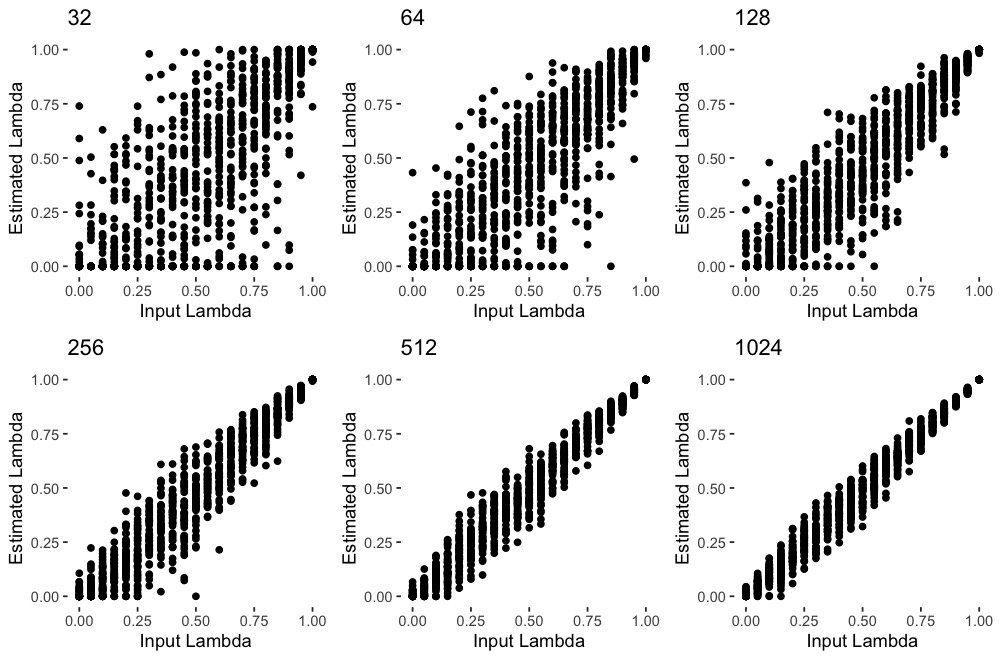
\includegraphics[width=0.95\linewidth]{Fig1}

\singlespacing \textbf{Figure 1}. Precision of Pagel's \(\lambda\)
across known levels of input phylogenetic signal (\(\lambda_{in}\)) on
phylogenies of various sizes. As phylogenies increase in size, variation
in \(\lambda_{in}\) decreases; however the precision is not constant
across the range of input levels (\(\lambda_{in}: 0 \to 1\)), and is
highest at intermediate levels of phylogenetic signal.

\newpage

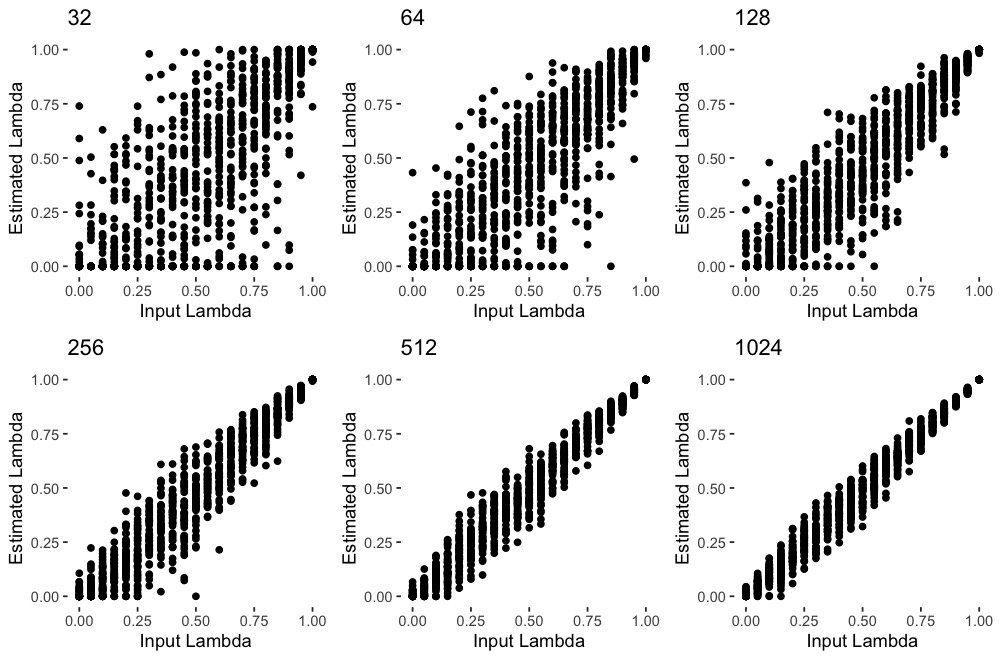
\includegraphics[width=0.95\linewidth]{Fig2}

\singlespacing \textbf{Figure 2}. Variation in estimates of phylogenetic
signal across input levels of phylogenetic signal. (A) Estimates of
Pagel's \(\lambda\) for data simulated on phylogenies with 128 taxa
(\(n=128\)), (B) Estimates of \(Z_K\) for data simulated on phylogenies
with 128 taxa (\(n=128\)), (C) Variance in the variation of
\(\lambda_{est}\) across input levels of phylogenetic signal, estimated
on phylogenies containing differing numbers of species. (D) Variance in
the variation of \(Z_K\) across input levels of phylogenetic signal,
estimated on phylogenies containing differing numbers of species.

\newpage

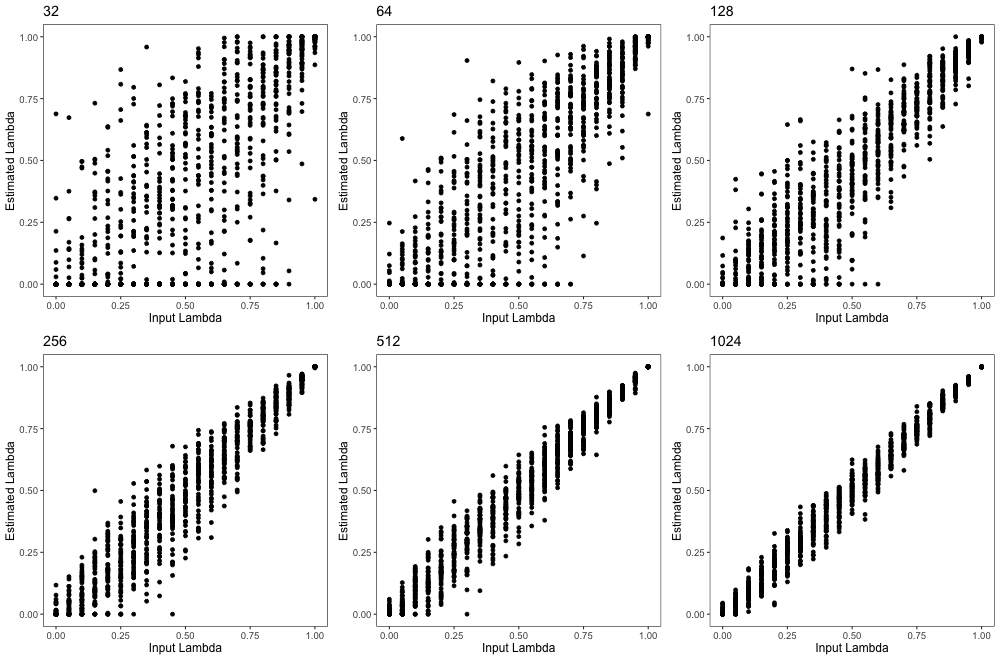
\includegraphics[width=0.95\linewidth]{Fig3}

\singlespacing \textbf{Figure 3}. Precision of Pagel's \(\lambda\) when
incorporated in phylogenetic regression (\(|Y\sim X\)), across known
levels of input phylogenetic signal (\(\lambda_{in}\)) on phylogenies of
various sizes. As phylogenies increase in size, variation in
\(\lambda_{in}\) decreases; however the precision is not constant across
the range of input levels (\(\lambda_{in}: 0 \to 1\)), and is highest at
intermediate levels of phylogenetic signal.

\newpage

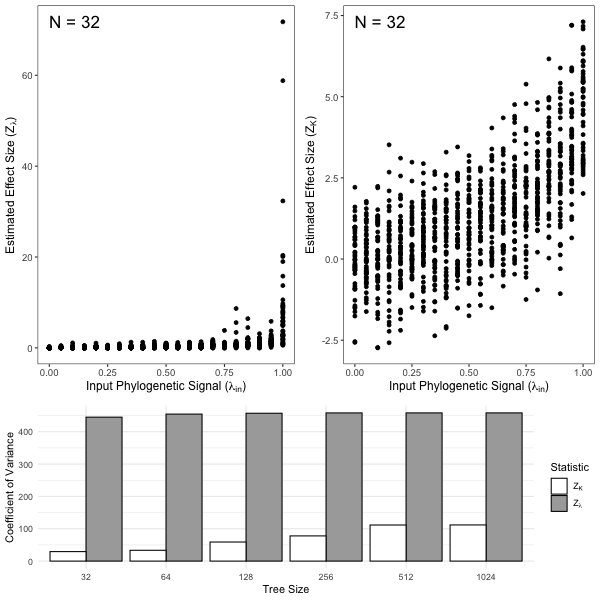
\includegraphics[width=0.95\linewidth]{Fig4}

\singlespacing \textbf{Figure 4}.Frequency of estimated lambda values
published in manuscripts in 2019. The majority of these values were
close to 0 or 1, and from phylogenies with fewer than 200 taxa.

\end{document}
